\chapter{Sistemos naudojimo scenarijus}

\section{Esamoji būklė}

Mokyklos būstinėje yra vienas nešiojamas kompiuteris su Windows operacine
sistema, kuriame laikomi visi aktualiu metu naudojami duomenys, bei 
prie jo prijungtas 
lazerinis spausdintuvas. Nuotolinio mokymo mokykla taip pat turi savo 
svetainę bei duomenų bazę su informacija apie moksleivius ir dėstytojus.
Darbuotojai dirba su savo asmeniniais kompiuteriais, kuriuose naudoja
įvairią programinę įrangą (pavyzdžiui, naudojamų operacinių sistemų 
sąraše yra „Windows XP“, „Windows 7“, „Ubuntu Linux“, „Xubuntu Linux“,
„Gentoo Linux“). Dauguma darbuotojų turi didelę darbo su biuro 
programomis patirtį.

\section{Scenarijaus aprašas}

\ref{fig:uml_usecase} diagramoje pavaizduota darbo su sistema UML schema.
\hfill \\

\begin{figure}[h!]
  \begin{center}
    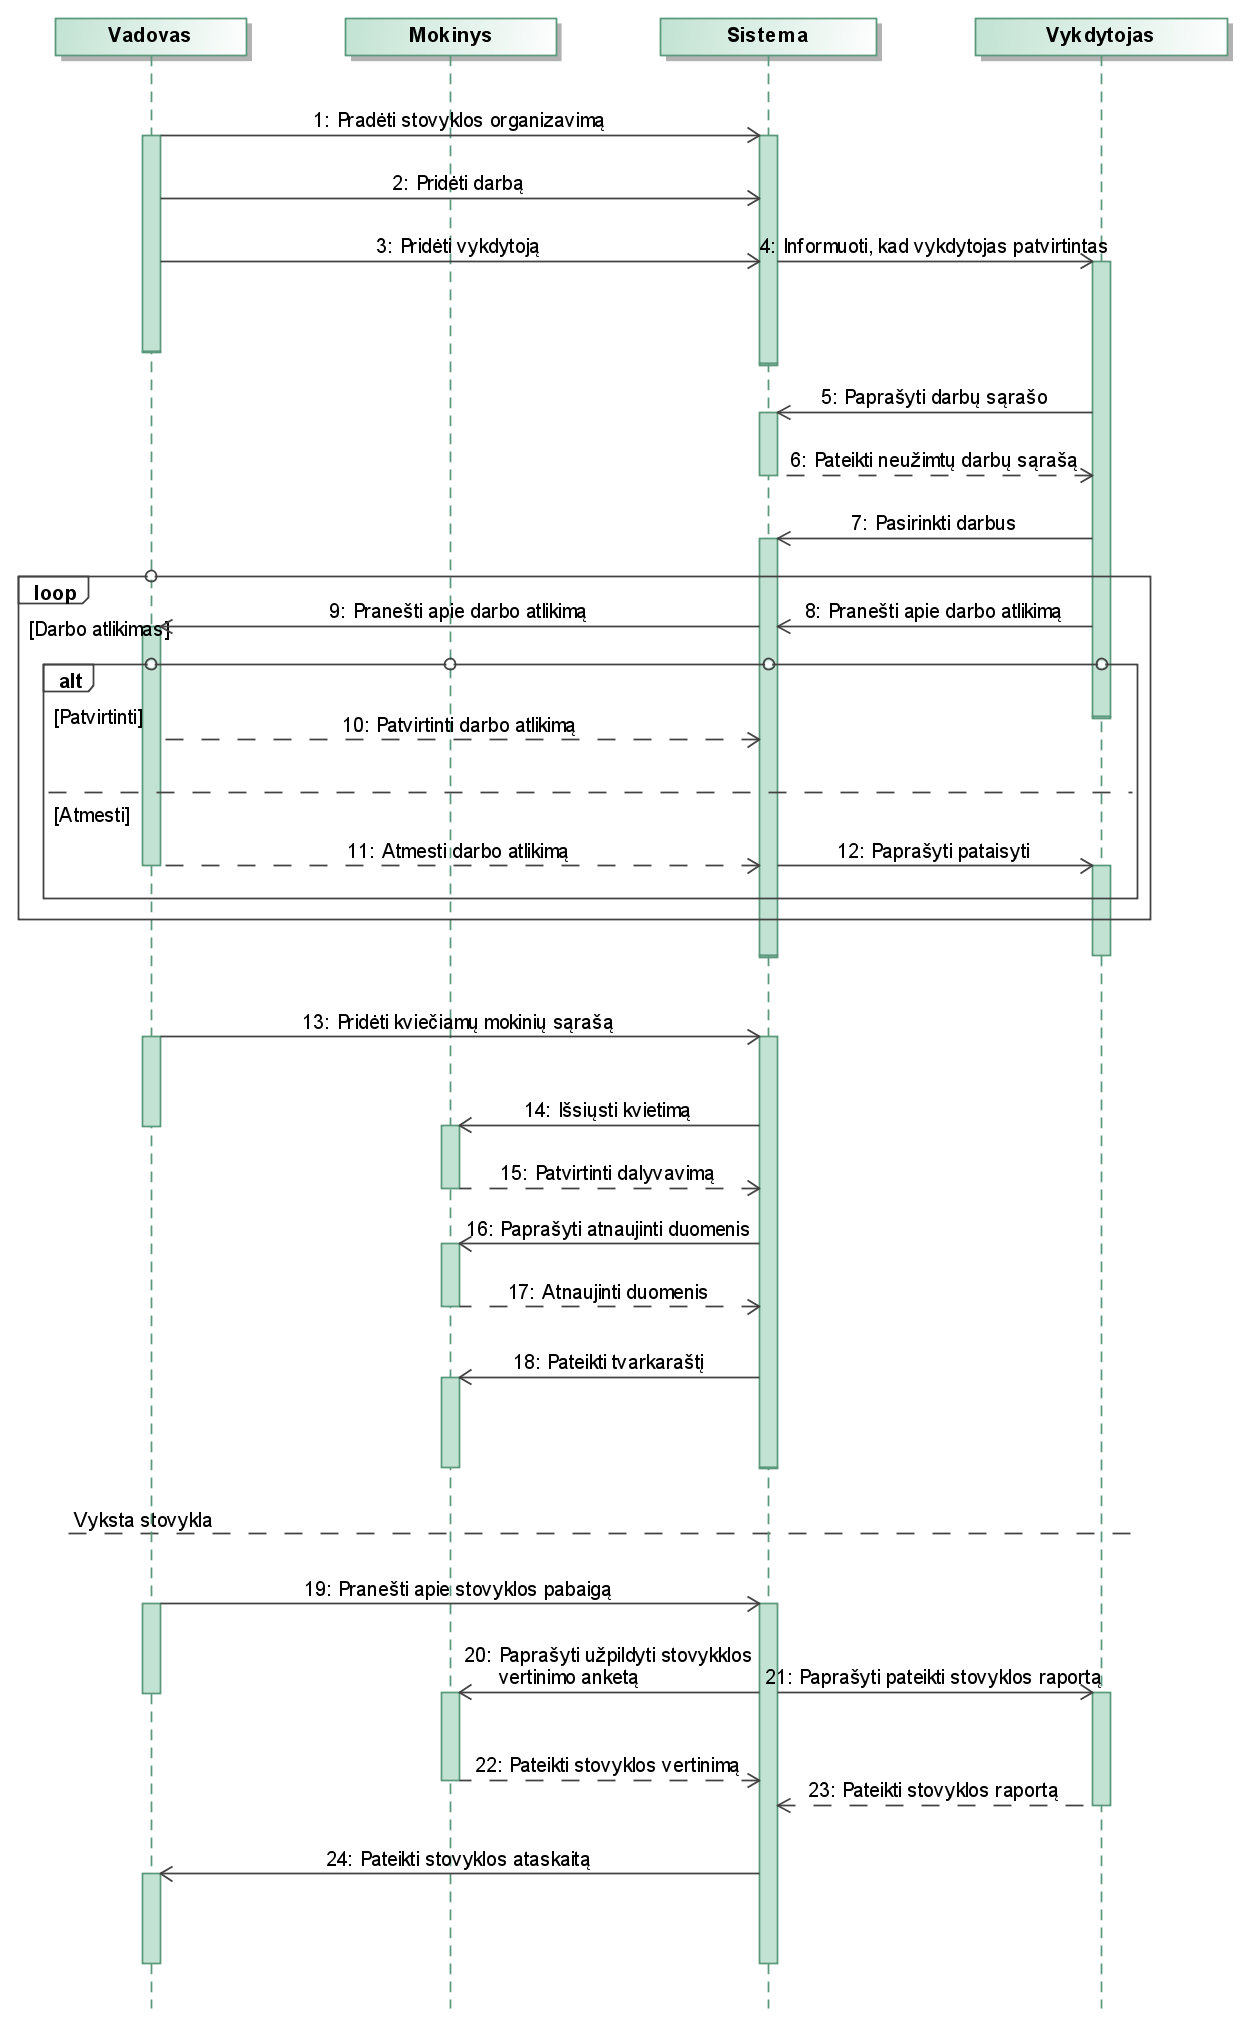
\includegraphics[scale=0.7]{images/Seka.png}
    \caption{UML schema vaizduojanti darbą su įdiegta sistema.}
  \end{center}
  \label{fig:uml_usecase}
\end{figure}

Vadovas duoda nurodymą sistemai pasiruošti stovyklos organizavimui.
Jis į sistemą įkelia darbų sąrašą, nurodydamas kiekvieno \glsdarbpozvnsg.  
Po to prideda vykdytojus, kurie atlikinės darbus iš darbų sąrašo. 
Vos pridėjus vykdytoją, sistema jį apie tai informuoja elektroniniu laišku. 

Vykdytojas, prisijungęs prie sistemos, gali peržiūrėti darbų sąrašą. 
Jis pasirenka darbą, kurį atlikinės. Baigęs pasirinkto darbo vykdymą, 
pažymi tą darbą kaip atliktą. Sistema informuoja vadovą apie darbo 
atlikimą ir paprašo tai patvirtinti. Vadovui atmetus darbo atlikimą, 
sistema informuoja apie tai vykdytoją, prašydama pataisyti darbą. 
Vykdytojui patvirtinus darbo pataisymą, sistema vėl prašo vadovo 
patvirtinti darbo kokybę. Taip daroma tol, kol vadovas ją patvirtina. 

Vėliau vadovas prideda kviečiamų moksleivių sąrašą. Sistema jiems 
išsiunčia kvietimus, reikalaudama patvirtinti, jog dalyvaus, 
arba pranešti, kad negalės atvykti. Patvirtinusių dalyvavimą 
moksleivių paprašoma patikslinti jų asmeninius duomenis, patvirtinti 
jų teisingumą. Kai užbaigiamas tvarkaraščio sudarymo procesas, 
sistema nusiunčia visiems dalyvausiantiems moksleiviams
tvarkaraščio kopiją.

Pasibaigus stovyklai, vadovas praneša apie tai sistemai. Ji moksleiviams
išsiuntinėja stovyklos vertinimo anketas bei darbų vykdytojų paprašo 
pateikti stovyklos raportą. Sistema, gavusi visus grįžtamuosius atsakymus,
suformuoja ataskaitą ir ją pateikia stovyklos vadovui.

\subsection{Darbo vietų aprašas}
\begin{enumerate}
  \item \emph{Vadovas}
	\begin{itemize}
	  \item Techninė įranga:
		\begin{enumerate}
			\item kompiuteris su internetu.
		\end{enumerate}
	  \item Programinė įranga:
		\begin{enumerate}
			\item operacinė sistema;
      \item interneto naršyklė.
		\end{enumerate}
	  \item Kvalifikaciniai reikalavimai:
		\begin{enumerate}
			\item kompiuterinio raštingumo pagrindai;
			\item sistemos „Skirstytuvas“ administravimo pagrindai.
		\end{enumerate}
	\end{itemize}

  \item \emph{Vykdytojas}
	\begin{itemize}
	  \item Techninė įranga:
		\begin{enumerate}
			\item kompiuteris su internetu.
		\end{enumerate}
	  \item Programinė įranga:
		\begin{enumerate}
			\item operacinė sistema;
      \item interneto naršyklė.
		\end{enumerate}
	  \item Kvalifikaciniai reikalavimai:
		\begin{enumerate}
			\item kompiuterinio raštingumo pagrindai;
			\item sistemos „Skirstytuvas“ naudojimo pagrindai.
		\end{enumerate}
	\end{itemize}
\end{enumerate}

\section{Priemonės scenarijui įgyvendinti}
\begin{enumerate}
  \item \Gls{virt_serv}
	\item Tinklo įranga
	\item Pašto serveris
	\item Duomenų bazių valdymo sistemos
	\item Interneto ryšio paslaugos
	\item Operacinės sistemos
	\item Darbuotojų apmokymas naudotis sistema
	\item Interneto svetainės vardo sritis .lt zonoje
\end{enumerate}
